This section describes the characterization of uncladded BCF-12 fibers, called no-clad fibers, from Saint-Gobain, which are the fibers selected for the TRITIUM experiment. These fibers are compared to single clad and multiclad BCF-12 fibers to quantify the influence of the clad in the relevant parameters of the scintillating fibers.

Although commercial clads are too thick for the TRITIUM experiment, the necessary low thickness clads could be developed. For example, clads with a thickness of the order of tens of nanometers can be achieved by electrodeposition techniques.

The difference between these three types of fibers is that uncladded fibers only consist of a polystyrene core with a refractive index of $1.60$ whereas, single clad fibers, have an acrylic clad (PMMA) of $30~\mu\meter$ thickness and a refractive index of $1.49$ and, multiclad fibers, have a second fluor-acrylic clad of $10~\mu\meter$ thickness  and a refractive index of 1.42.

%The first measurement that was made is the measurement of the diameter of the fiber. It is important because scintillating molecules are only present in the polystyrene core and we need to know whether the entire polystyrene core is the same size or not. Three different samples of each type of fiber were measured and the results are presented in Table \ ref {}.

%TABLAAA DIAMETROOOS

%Therefore, we can see that all fibers have the same external size, which means that the diameter of the polystyrene core is smaller for single clad fibers ($0.97~\mm$) and even smaller for multiclad fibers ($0.96~\mm$). It is an important result since...

This characterization was carried out at the level of a single scintillating fiber. The parameters measured for each fiber type were the fiber collection efficiency and the uncertainty of the fiber response due to the conditioning process. The reference magnitude employed for the characterization is the rate of photons that reach the active area of the photosensor. To measure this magnitude, a calibrated R8520-06SEL PMT was used, whose quantum efficiency at the working wavelength, $29.76\%$, was measured by Hamamatsu. The PCB described in section \ref{subsubsec:PMTsElectronicalSystem} was used for working without the PMT internal gain and the PMT output current was measured by a Keithley 6487 Picoammeter/Voltage Source. The photons rate was obtained from the current measurement using the equation \ref{eq:NumPhotonsFromIntensityPMT} with $QE=0.2976$ and $CE=1$. A simplified scheme of the used set up is shown in Figure \ref{fig:SetUpFiberCharacterization}.

\begin{figure}[h]
\centering
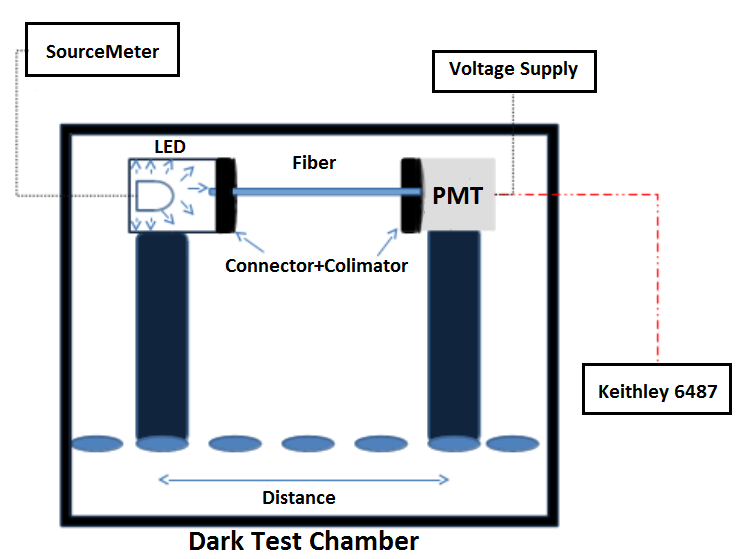
\includegraphics[scale=0.6]{4ResearchAndDevelopments/41Fibers/SetUp_Fiber_Characterization.png}
\caption{Set up used for fiber characterization.\label{fig:SetUpFiberCharacterization}}
\end{figure}

This setup consists of an optical structure in which a LED and a PMT are fixed to a user set distance between them. A LED435-03 from Roithner LaserTechnik Gmbh \cite{LEDRLT}, simulated the light emission by the fibers. The emission spectrum of the LED, given in Figure \ref{fig:LEDSpectrumTritium}, was experimentaly measured by a spectrometer and fitted to a Gaussian function. The LED emission peak is at $433.9~\nano\meter$ with a FWHM of $18.4~\nm$. 

\begin{figure}[h]
\centering
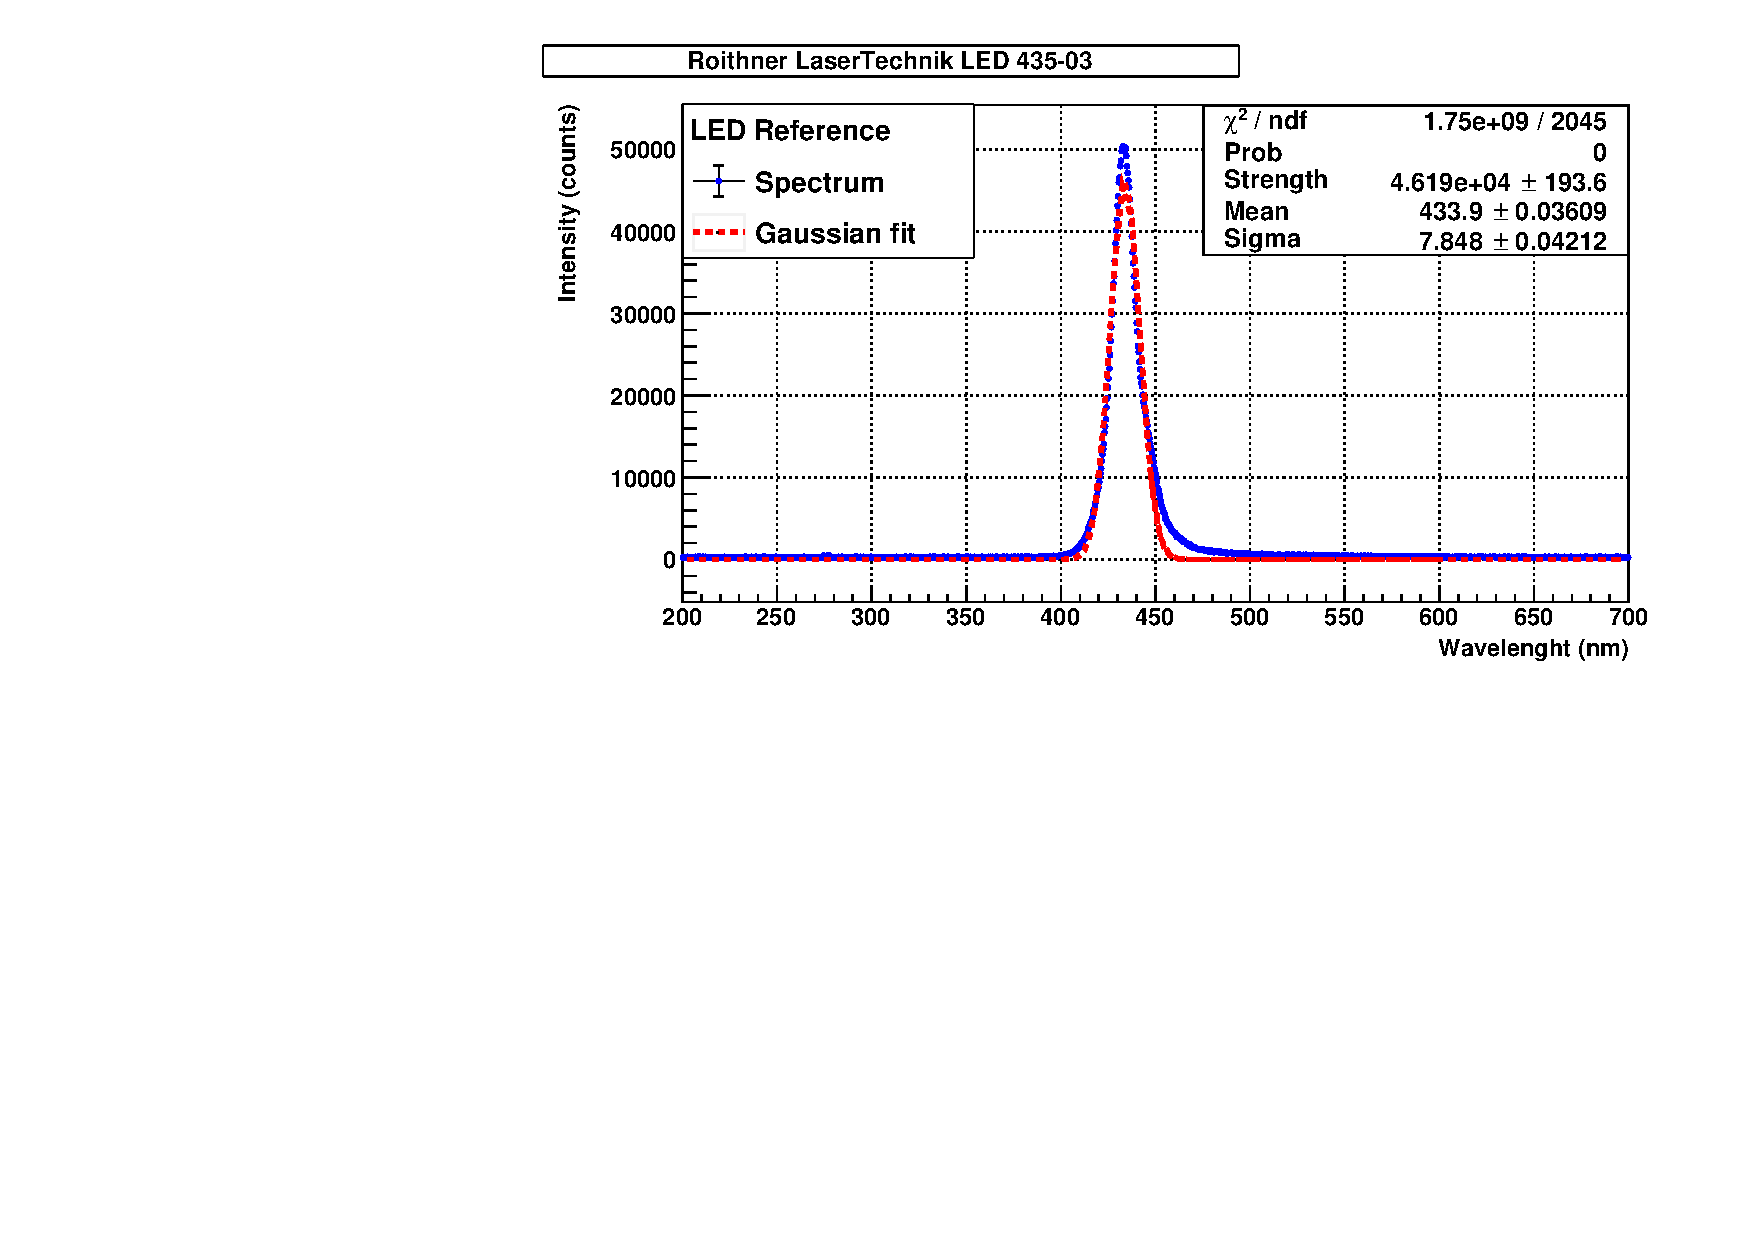
\includegraphics[scale=0.6]{4ResearchAndDevelopments/41Fibers/LED_TRITIUM.pdf}
\caption{Emission spectrum measured for the LED model 435-03 from Roithner LaserTechnik Gmbh Company.\label{fig:LEDSpectrumTritium}}
\end{figure}

The fiber was fixed between the LED and the PMT. The length of the fiber was $20~\cm$. Optical grease \cite{OpticalGrease} was used for optimal coupling between the fiber and the PMT. Two collimators were used to ensure that only photons detected from the LED were detected in the PMT. Two FH-ST\footnote{FH-ST is a quick assembly connector for $1~\mm$ POF, Plastic Optical Fiber} connectors from RoHS company \cite{}, were used to fix the fiber to the system. 